\section{Pretraining}
\label{sec:pretraining}

In this section, we provide details on the pretraining of \ourmodel. Specifically, we detail the architecture, NVFP4 pretraining recipe, data, and hyperparameters used for \ourbasemodel. We also share details on the long context extension phase, model training instabilities, and benchmark accuracies.

\subsection{Model Architecture}
\label{sec:architecture}

\ourmodel uses the same hybrid Mamba-Attention Mixture-of-Experts (MoE) architecture as Nemotron 3 Super~\citep{nvidia2026nemotron3superopen}, extended to 550B total parameters with 55B active parameters per token. As with Nemotron 3 Super, we leverage LatentMoE~\citep{latentmoe_tr} for MoE layers and native Multi-Token Prediction for inference acceleration with two heads during pre-training. Both MTP heads share the same parameters to enable robust autoregressive drafting as described in~\cite{nvidia2026nemotron3superopen} and consist of a single attention layer followed by a single MoE layer. The layer pattern and configuration for \ourmodel are shown in Figure~\ref{fig:layer-pattern} and Table~\ref{table:model_arch}, respectively.

\begin{figure}[!ht]
\centering
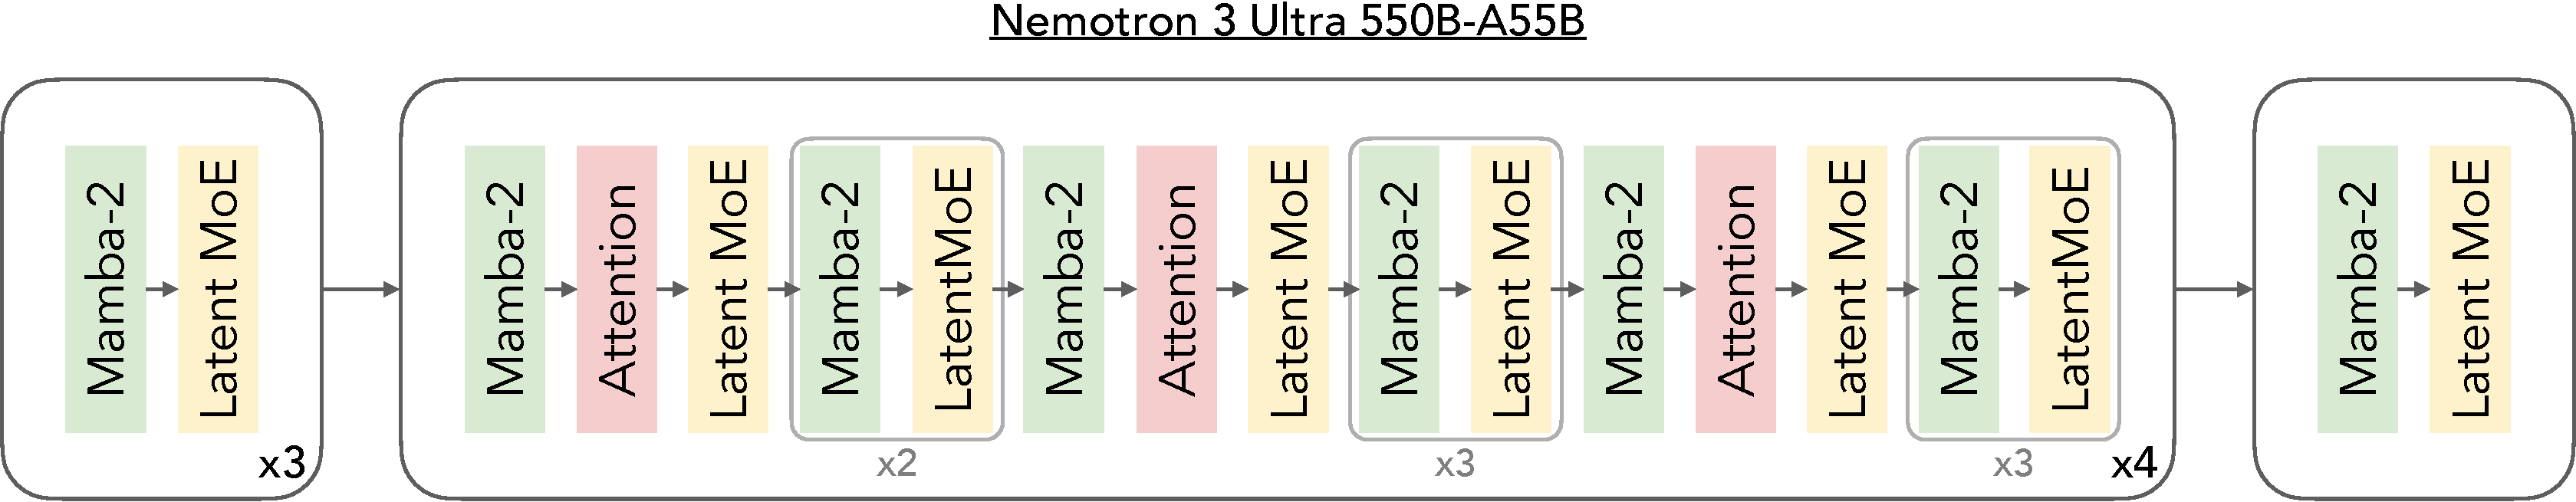
\includegraphics[width=0.9\linewidth]{figures/ultrav3.pdf}
\caption{\ourmodel layer pattern. Similar to Nemotron 3 Super, we use a hybrid Mamba-Attention architecture scaled sparsely using LatentMoE layers.}
\label{fig:layer-pattern}
\end{figure}


\begin{table*}[!ht]\small\centering
\renewcommand{\arraystretch}{1.2}
\setlength{\tabcolsep}{10pt}
\begin{tabular}{l|c}
\toprule
\textbf{Configuration} & \textbf{\ourmodel} \\
\midrule
Total Layers & 108 \\
Model Dimension  & 8192 \\
\midrule
Q-Heads ($n_{q}$) & 64 \\
KV-Heads ($n_{kv}$) & 2 \\
Head Dimension & 128 \\
\midrule
Mamba State Dimension & 128 \\
Mamba Groups & 8  \\ 
Mamba Heads & 256 \\
Mamba Head Dimension & 64 \\ 
\midrule
Expert Hidden Dimension & 5120 \\
Shared Expert Intermediate Size & 10240 \\
Total Experts per Layer & 512 \\
Top-$k$ (Activated Experts) & 22 \\
\midrule
MoE Latent Size & 2048 \\
\midrule
MTP layers (shared weight) & 2 \\ 
\bottomrule
\end{tabular}
\caption{\ourmodel Architecture Dimensions.}
\label{table:model_arch}
\end{table*}


\subsection{NVFP4 Pretraining}

\begin{figure*}[!h]
    \centering
    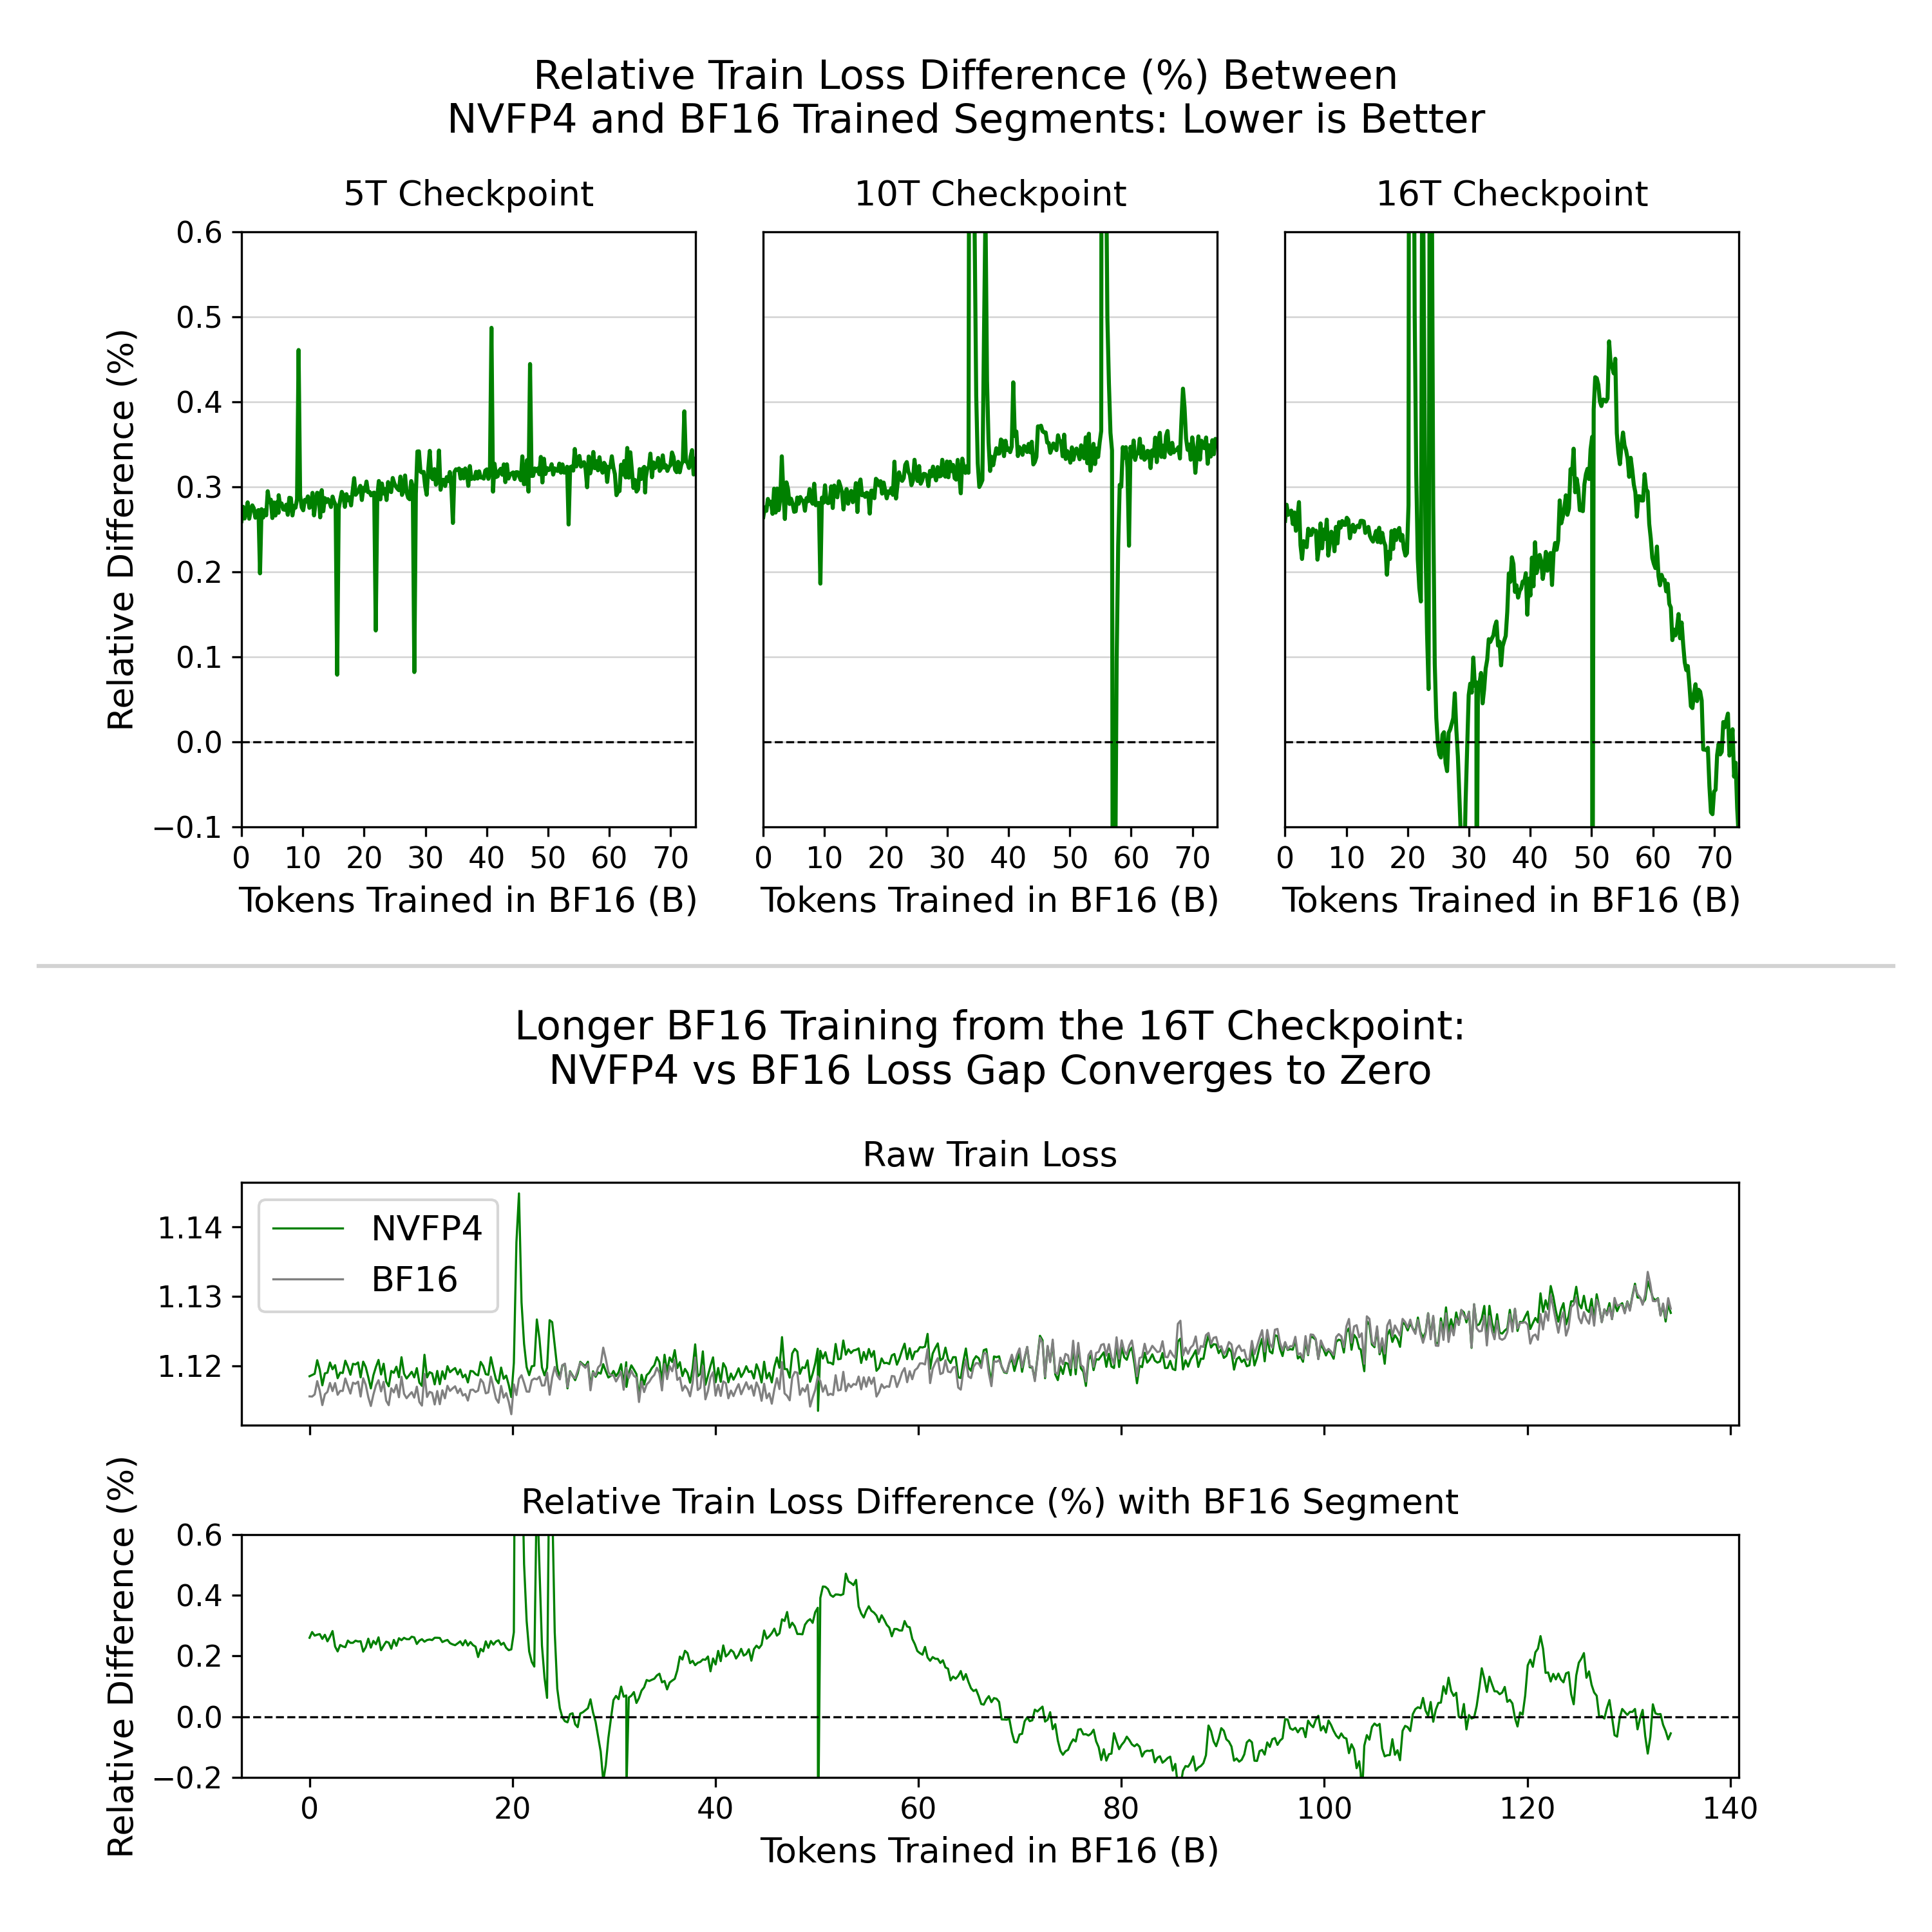
\includegraphics[width=0.8\linewidth]{figures/NVFP4_Pretrain_Ultra3_Figure.png}
    \caption{Top: Ablation studies switching all tensors to BF16 from 5T, 10T, 16T token checkpoints, respectively, shown as relative percent difference in train loss between NVFP4 and BF16. The starting loss gap for each ablation study was within 0.28\%. After 74B tokens of BF16 training, the loss gap increases to 0.33\% and 0.34\% from the 5T and 10T checkpoints, and decreases to 0.03\% from the 16T checkpoint. Bottom: Longer training in BF16 from the 16T token checkpoint. Raw train loss shows similar pattern of divergence for both BF16 and NVFP4 models. Relative difference in train loss (\%) converges toward zero during the training divergence. Switching all tensors to BF16 did not resolve the training divergence.}
    \label{fig:nvfp4_pretrain}
\end{figure*}

We trained \ourmodel using the same NVFP4 pretraining recipe as Nemotron 3 Super \cite{nvidia2026nemotron3superopen}, leveraging Transformer Engine's open-source cuBLAS NVFP4 GEMM kernels for fprop, dgrad, and wgrad. NVFP4 layers use the E2M1 datatype with two-dimensional block quantization on weights, Random Hadamard Transforms on inputs to wgrad, and stochastic rounding on gradients \cite{nvidia2025pretraininglargelanguagemodels}. We kept the final 15\% of the network (16 layers), Mamba output projections, latent projections, QKV and attention projections, MTP layers, and embedding layers in higher precision following \cite{nvidia2025nvidianemotron3efficient, nvidia2026nemotron3superopen}. To our knowledge, this is the largest-scale demonstration of stable and accurate NVFP4 training to date.

To monitor training health, we branched ablations from checkpoints at 5T, 10T, and 16T tokens, switched all tensors to BF16, and continued pretraining for 74B tokens. We tracked the relative train loss difference between BF16 segments and \ourmodel (NVFP4). As seen in prior work, switching all tensors to BF16 substantially recovers the high-precision loss, providing a proxy for high-precision training \cite{nvidia2025pretraininglargelanguagemodels}.  These three ablation studies on \ourmodel showed a relative train loss gap against the BF16 segments below 0.4\% on average (Figure \ref{fig:nvfp4_pretrain}, top), which is lower than NVFP4 vs. BF16 train loss gaps observed on smaller model variants \cite{nvidia2025nvidianemotron3efficient}. The relative train loss gap averaged over the first 5B tokens of BF16 training was 0.27\%, 0.28\%, and 0.25\% starting from the 5T, 10T, and 16T checkpoints, respectively. After 74B tokens of BF16 training, the relative train loss gap increases to 0.33\% and 0.34\% from the 5T and 10T checkpoints, and decreases to 0.03\% from the 16T checkpoint, averaged over the final 5B tokens. Switching all tensors to BF16 did not resolve the training divergence discussed in section \ref{sec:stability} (Figure \ref{fig:nvfp4_pretrain}, bottom).

\subsection{Pretraining Data}

%\todo{PIC {\bf Markus}}

In this section, we describe the new data that we added to pretraining since Nemotron 3 Super~\citep{nvidia2026nemotron3superopen}. We are releasing these new datasets on HuggingFace.\footnote{\href{https://huggingface.co/datasets/nvidia/Nemotron-Pretraining-Code-v3}{\texttt{Nemotron-Pretraining-Code-v3}}, \href{https://huggingface.co/datasets/nvidia/Nemotron-Pretraining-Legal-v1}{\texttt{Nemotron-Pretraining-Legal-v1}}, \href{https://huggingface.co/datasets/nvidia/Nemotron-Pretraining-Specialized-v1.2}{\texttt{Nemotron-Pretraining-Specialized-v1.2}}}

%\footnote{\url{https://huggingface.co/datasets/nvidia/Nemotron-Pretraining-Code-v3}, \url{https://huggingface.co/datasets/nvidia/Nemotron-Pretraining-Legal-v1}, \url{https://huggingface.co/datasets/nvidia/Nemotron-Pretraining-Specialized-v1.2}}


\subsubsection{Code refresh}

We refreshed our raw source code data from GitHub, adding 173B new tokens with a cut-off date of September 30, 2025.

\subsubsection{Nemotron-Pretraining-Multiple-Choice and Nemotron-Pretraining-Generative}
%\todo{Dan Su}


We generated large-scale, task-seeded synthetic Q\&A data from the training splits of many public datasets spanning a wide range of domains, including STEM, factual knowledge, commonsense reasoning, logical reasoning, math, code, reading comprehension, and multilingual QA.
%\footnote{acp\_bench; babi; gsm8k; hendrycks\_math; IFEval; MedText; mediqa\_qa; mlqa; MMLU-Pro; mmlu-pro-plus; MMLU-ProX; nq\_open; tinyGSM8k; truthfulqa-multi; MATH-lighteval; mmlu; awesome-chatgpt-prompts; super\_glue; Into the Unknown; AI2 ARC (AI2 Reasoning Challenge); BLiMP (Benchmark of Linguistic Minimal Pairs); CommonSenseQA; GLUE; HeadQA; Hendrycks Ethics; Memo Trap; modus-tollens; NeQA; pattern-matching-suppression; mastermind\_24\_mcq\_random; mastermind\_24\_mcq\_close; quote-repetition; redefine-math; Repetitive Algebra; sig-figs; MC-TACO; MedConceptsQA; MMLU\_dataset; OpenbooksQA; PIQA (Physical Interaction Question Answering); SocialIQA; SuperGLUE; tinyAI2\_arc; tinyMMLU; tinyWinogrande; TruthfulQA; WebQuestions; Winogrande; GPQA; MBPP}.
Held-out test splits were not used for data generation. The source benchmark training examples were used as seeds to capture task structure, domain, difficulty, and answer format, while the generated examples were newly synthesized to preserve the underlying capability being tested rather than reproduce evaluation instances.

We organize the resulting data into two dataset families: Nemotron-Pretraining-Multiple-Choice, which contains synthetic questions with answer options and normalized correct answers, and Nemotron-Pretraining-Generative, which contains open-ended Q\&A examples with free-form answers. For both formats, we generate answer-enriched samples that include task-relevant knowledge, reasoning, or explanatory context when appropriate. We apply formatting checks, schema validation, deduplication, and task-specific filtering to improve data quality. These datasets are designed to promote cross-task capability transfer by exposing the model to diverse task formats, reasoning patterns, and knowledge domains during pretraining.

To validate the quality of this data, we conducted a 100B-token phase-3 continued-pretraining ablation on a Nemotron-family base checkpoint. Adding the benchmark-oriented synthetic data improved MMLU-Pro from 64.8 to 66.6, average code from 73.2 to 75.1, commonsense understanding from 72.9 to 74.5, and GPQA from 30.8 to 41.9, while average math remained stable (87.6 to 87.9).

\subsubsection{Nemotron-Pretraining-Fact-Seeking}

This dataset contains fact-seeking questions generated from Finewiki~\citep{penedo2025finewiki}. We generate the questions in two stages:
extracting informative, factual statements from Finewiki articles, and prompting Qwen3-30B-A3B-Instruct-2507 with each statement and its original context to generate either a short-answer or multiple-choice question.

To verify the usefulness of the data, we conducted an ablation study using an intermediate checkpoint from Nemotron 3 Nano pretraining. We injected the fact-seeking data during the final 100B tokens of training, improving accuracy on SimpleQA from 40.24 to 50.16. Since we converted SimpleQA questions into multiple-choice format for easier evaluation, these scores are not directly comparable to the original SimpleQA scores.

\subsubsection{Nemotron-Pretraining-Moral-Scenarios}

In the SFT data we previously released\footnote{\url{https://huggingface.co/datasets/nvidia/Nemotron-Pretraining-SFT-v1}}, we included multiple-choice questions about moral scenarios. These questions were constructed using situations and norms from Moral Stories~\citep{emelin-etal-2021-moral} and actions from Social Chemistry~\citep{forbes-etal-2020-social}. In this work, we sampled a subset of these examples and created a chain-of-thought version using Qwen3-235B-A22B-Thinking-2507.

\subsubsection{Nemotron-Pretraining-Legal}

We curated and generated a number of datasets targeting the legal domain as follows.

\begin{itemize}
    \item Datasets extracted from HTML files
    \begin{itemize}
        \item \textbf{Nemotron-Pretraining-Legal-California-Code-Of-Regulations}: California Code of Regulations\footnote{\url{https://govt.westlaw.com/calregs/Index}}, excluding Title 6 and Title 24.
        \item \textbf{Nemotron-Pretraining-Legal-NYCourts-Judicial-Ethics-Opinions}: New York Court Judicial Ethical Opinions\footnote{\url{https://www.nycourts.gov/ipjudicialethicsopinions}}.
        \item \textbf{Nemotron-Pretraining-Legal-eCFR}: Code of Federal Regulations\footnote{\url{https://www.ecfr.gov/}}.
    \end{itemize}

    \item LLM-cleaned datasets
    \begin{itemize}
        \item \textbf{Nemotron-Pretraining-Legal-Case-Law-Summary}: 5.4M summaries generated from a filtered version of Caselaw\footnote{\url{https://huggingface.co/datasets/common-pile/caselaw_access_project_filtered}} using Qwen3-235B-A22B-Instruct-2507.
    \end{itemize}

    \item Reformatted datasets
    \begin{itemize}
        \item \textbf{Nemotron-Pretraining-Legal-CaseHOLD}: We transformed the CaseHOLD dataset\footnote{\url{https://huggingface.co/datasets/casehold/casehold}} into a multiple-choice format.
        \item \textbf{Nemotron-Pretraining-Legal-Contract-NLI}: For each non-disclosure agreement in the ContractNLI dataset\footnote{\url{https://stanfordnlp.github.io/contract-nli/}}, we extracted the annotated hypotheses, answers, and evidence statements and appended them to the source document.
    \end{itemize}

    \item Synthetic datasets
    \begin{itemize}
        \item \textbf{Nemotron-Pretraining-Legal-Canadian-Case-Law-Outcome}: We identified passages from the CHRT, RPD, RAD, and RLLR subsets of the Canadian Case Law dataset\footnote{\url{https://huggingface.co/datasets/a2aj/canadian-case-law}} that clearly state the outcome of an appeal (allowed, dismissed, or other), as well as random passages that do not include the outcome using Qwen3-235B-A22B-Instruct-2507.
        \item \textbf{Nemotron-Pretraining-Legal-Definition-Classification}: From Caselaw, we extracted passages containing defining language as positive examples using Qwen3-235B-A22B-Instruct-2507 and randomly selected passages not containing defining language as negative examples. We use these passages to construct questions that classify whether a text from a judicial opinion defines a term.
        \item \textbf{Nemotron-Pretraining-Legal-Diversity-Jurisdiction}: This dataset contains questions that ask whether complete diversity exists between plaintiffs and defendants. The questions are generated from templates using random person names sampled from Nemotron Persona, along with states and causes of action sampled from two predefined lists. We also rephrase questions using Qwen3-235B-A22B-Instruct-2507 to increase diversity.
        \item \textbf{Nemotron-Pretraining-Legal-Function-Of-Decision}: We randomly sampled paragraphs from Caselaw documents and prompted Qwen3-235B-A22B-Instruct-2507 to classify its function into 7 pre-defined categories (facts, procedural history, issue, rule, analysis, conclusion, decree). We further balanced the number of examples for each category.
        \item \textbf{Nemotron-Pretraining-Legal-GlobalCit}: This dataset contains questions related to global nationality laws, converted from the GLOBALCIT dataset\footnote{\url{https://globalcit.eu/databases/globalcit-citizenship-law-dataset}} based on its codebook. We rephrased each question into three different version using Qwen3-235B-A22B-Instruct-2507.
        \item \textbf{Nemotron-Pretraining-Legal-LegalBench-CUAD-v2}: This dataset contains questions that ask whether a clause is a specific type of clause in a contract defined in the Contract Understanding Atticus Dataset (CUAD)\footnote{\url{https://www.atticusprojectai.org/cuad/}}. Using Qwen3-235B-A22B-Instruct-2507, we cleaned raw CUAD contracts shorter than 8k tokens, extracted the first qualifying clause of each type from each contract, and generated a negative example from each extracted clause. For some categories (\texttt{affiliate\_license\_licensor}, \texttt{affiliate\_license\_licensee}, \texttt{post\_termination\_services}, \texttt{exclusivity}, \texttt{effective \_date}, \texttt{non\_disparagement}, \texttt{unlimited\_all\_you\_can\_eat\_license}) where the identification accuracy is low, we composed longer prompts with detailed instructions based on the labeling handbook to extract qualifying clauses.
        \item \textbf{Nemotron-Pretraining-Legal-ToS-Clause-Understanding}: This dataset contains terms of service clause understanding questions. We generated a relevant legal question about each clause from the TOS Dataset\footnote{\url{https://huggingface.co/datasets/CodeHima/TOS_Dataset}} using Qwen3-235B-A22B-Instruct-2507.
        \item \textbf{Nemotron-Pretraining-Legal-ToSDR-QA}: This dataset contains Yes/No questions that address different sections or issues covered by each contract in the ToSDR Terms of Service Corpus\footnote{\url{https://www.kaggle.com/datasets/sonu1607/tosdr-terms-of-service-corpus}} using Qwen3-235B-A22B-Instruct-2507.
        \item \textbf{Nemotron-Pretraining-Legal-eCFR-QA}: This dataset contains DiverseQA-like data generated from the Code of Federal Regulations. We generated a variety of question from CFR excerpts and evaluate the correctness of each answer using Qwen3-235B-A22B-Instruct-2507.
    \end{itemize}

\end{itemize}

We conducted an ablation study using an intermediate checkpoint from Nemotron 3 Nano pretraining, an MoE with 30B total and 3B active parameters. Starting from a 14.9T token checkpoint, we trained for an additional 100B tokens using a phase 2 blend and evaluated models on over 100 subtasks in LegalBench. The experiment results show that these legal-specific datasets substantially improve our model’s accuracy on LegalBench tasks across multiple categories, boosting the average accuracy from 64.6 to 74.7.

% \paragraph{Datasets extracted from HTML files}

% \begin{itemize}
%     \item \textbf{Nemotron-Pretraining-Legal-California-Code-Of-Regulations}: California Code of Regulations.
%     \item \textbf{Nemotron-Pretraining-Legal-NYCourts-Judicial-Ethics-Opinions}: New York Court Judicial Ethical Opinions.
%     \item \textbf{Nemotron-Pretraining-Legal-eCFR}: Code of Federal Regulations.
% \end{itemize}

% \paragraph{LLM-cleaned datasets}

% \begin{itemize}
%     \item \textbf{Nemotron-Pretraining-Legal-Case-Law-Summary}: 5.4M case law summaries.
% \end{itemize}

% \paragraph{Reformatted datasets}

% \begin{itemize}
%     \item \textbf{Nemotron-Pretraining-Legal-CaseHOLD}: Reformatted CaseHOLD dataset.
%     \item \textbf{Nemotron-Pretraining-Legal-Contract-NLI}: Reformatted ContractNLI dataset.
% \end{itemize}

% \paragraph{Synthetic datasets}

% \begin{itemize}
%     \item \textbf{Nemotron-Pretraining-Legal-Canadian-Case-Law-Outcome}: Indicate the outcome given an excerpt from a Tax Court of Canada decision. Generated from the CHRT, RPD, RAD, and RLLR subsets of the a2aj/canadian-case-law dataset. We only use these four because the use of any other subsets for commercial purposes is not allowed.
%     \item \textbf{Nemotron-Pretraining-Legal-Definition-Classification}: Classify whether a text from a judicial opinion defines a term. Generated from CaseLaw. We use Qwen3-235B-A22B-Instruct-2507 to extract passages containing defining language as positive examples and randomly pick passages not containing defining language as negative examples.
%     \item \textbf{Nemotron-Pretraining-Legal-Diversity-Jurisdiction}: Classify whether there is complete diversity between plaintiffs and defendants. Template-based generation using random person names sampled from Nemotron Persona and states and causes of action sampled from two lists. A rephrased version is generated using Qwen3-235B-A22B-Instruct-2507.
%     \item \textbf{Nemotron-Pretraining-Legal-Function-Of-Decision}: Classify the function of a decision paragraph into 7 pre-defined categories. Generated from CaseLaw. We sample up to 2 sentences from each case and use Qwen3-235B-A22B-Instruct-2507 to classify the function of each sentence (the surrounding sentences are provided as context). We balance the number of examples for each category.
%     \item \textbf{Nemotron-Pretraining-Legal-GlobalCit}: Questions related to global nationality laws. Converted from the GLOBALCIT dataset based on its codebook. We then use Qwen3-235B-A22B-Instruct-2507 to rephrase the questions.
%     \item \textbf{Nemotron-Pretraining-Legal-LegalBench-CUAD-v2}: Classify whether a clause is a specific type of clause in a contract. Using Qwen3-235B-A22B-Instruct-2507, we clean raw CUAD contracts shorter than 8k tokens, extract the first qualifying clause of each type from each contract, and generate a negative example from each clause. For some categories (\texttt{affiliate\_license\_licensor}, \texttt{affiliate\_license\_licensee}, \texttt{post\_termination\_services}, \texttt{exclusivity}, \texttt{effective\_date}, \texttt{non\_disparagement}, \texttt{unlimited\_all\_you\_can\_eat\_license}) where the accuracy is low, we compose longer prompts with detailed instructions to extract qualifying clauses.
%     \item \textbf{Nemotron-Pretraining-Legal-ToS-Clause-Understanding}: Terms of service clause understanding questions. We generate relevant legal question about each clause from the CodeHima/TOS\_Dataset dataset using Qwen3-235B-A22B-Instruct-2507.
%     \item \textbf{Nemotron-Pretraining-Legal-ToSDR-QA}: Yes/No questions generated from ToSDR. We clean Terms of Services documents from the ToSDR dataset and Yes/No questions that address different sections or issues covered by each contract using Qwen3-235B-A22B-Instruct-2507.
%     \item \textbf{Nemotron-Pretraining-Legal-eCFR-QA}: DiverseQA-like data generated from the Code of Federal Regulations. We generate a variety of question from CFR excerpts and evaluate the correctness of each answer using Qwen3-235B-A22B-Instruct-2507.
% \end{itemize}



% TODO: Include more detailed ablation table for the legal datasets?




\subsubsection{Data Mixture and Ordering}

The data mixtures used to train \ourmodel are an adaptation of the data mixtures used to train Nemotron 3 Super and Nano \citep{nvidia2025nemotron3nanoopen, nvidia2026nemotron3superopen}, and incorporate new and refreshed datasets. Following \citet{feng2024maximizedataspotentialenhancing}, we design our data mixtures to balance diversity and quality. We adopt the proposed two-phase curriculum and transition from a data mixture which biases dataset diversity (phase 1) to a data mixture which biases dataset quality (phase 2). This transition occurs after ${\sim}15$ trillion tokens corresponding to ${\sim}75\%$ of pretraining. We present the high-level breakdown for the phase 1 and phase 2 data mixtures in Figure~\ref{fig:data-mixtures}. More detail on quality estimation and dataset composition are available in \citet{feng2024maximizedataspotentialenhancing} and the Nemotron 3 Super and Nano reports \citep{nvidia2025nemotron3nanoopen,nvidia2026nemotron3superopen}.

The pretraining corpus spans 19 high level categories across both data mixtures. The largest component, accounting for ${\sim}49\%$ of phase 1 tokens and ${\sim}38\%$ of phase 2 tokens, consists of quality-filtered and synthetic web crawl data: crawl-medium, crawl-medium-high, crawl-high, syn-crawl-medium, and syn-crawl-high. Other categories include finepdfs \citep{kydlicek2025finepdfs} which we quality-filter and upweight for inclusion in phase 2, math data \citep{mahabadi2025nemotronccmath133billiontokenscalehigh,akter2025mindmathinformedsynthetic}, code data, Nemotron-CC-Code, Wikipedia, academic texts, legal data, multilingual data spanning 11 languages (Arabic, Chinese, French, German, Hebrew, Hindi, Italian, Japanese, Korean, Portuguese, Spanish), Crawl++, and synthetic SFT-style data. Crawl++ consists of OpenWebText, BigScience \citep{laurencon2023bigsciencerootscorpus16tb}, and Reddit datasets. The SFT-style data, subcategorized as sft-code, sft-stem, and sft-general, we include per \citet{akter2026frontloading} who demonstrate its effectiveness.


\begin{figure}[!t]
    \centering
    \begin{subfigure}[b]{0.49\textwidth}
        \centering
        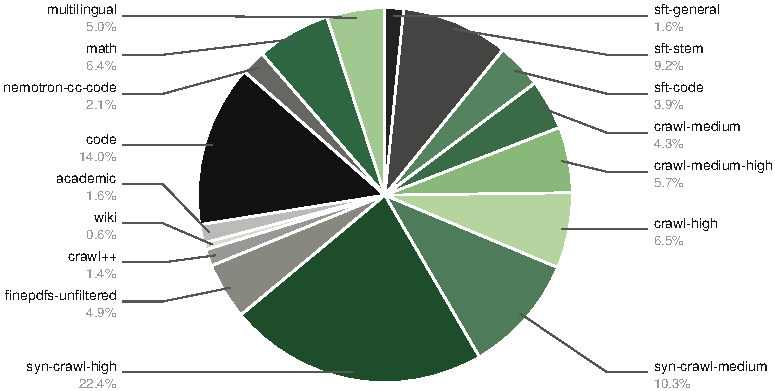
\includegraphics[width=\linewidth]{figures/data_mixture_phase1.pdf}
        \caption{Data mixture of phase 1}
        \label{fig:data-mixture-phase1}
    \end{subfigure}
    \hfill
    \begin{subfigure}[b]{0.49\textwidth}
        \centering
        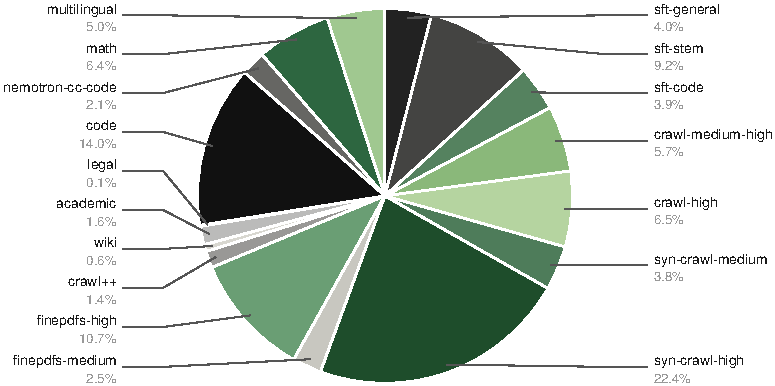
\includegraphics[width=\linewidth]{figures/data_mixture_phase2.pdf}
        \caption{Data mixture of phase 2}
        \label{fig:data-mixture-phase2}
    \end{subfigure}
    \caption{The data mixtures for both pretraining phases. We design the phase 1 data mixture to have a bias for diversity and the phase 2 data mixture to have a bias for quality.}
    \label{fig:data-mixtures}
\end{figure}

\subsection{Hyperparameters}
\label{sec:hyperparameters}
We follow the same training recipe and hyperparameters as Nemotron 3 Super~\citep{nvidia2026nemotron3superopen}, with a few adjustments: For \ourmodel we use a Warmup-Stable-Decay (WSD) learning rate schedule over a total horizon of 20 trillion tokens. We warmup the learning rate for 200 billion tokens to a peak value of $2.5 \times 10^{-4}$. For the final 5 trillion tokens we then decay the learning rate according to a minus-sqrt decay schedule to a minimum of $2.5 \times 10^{-6}$. 
As in Nemotron 3 Super, we used offline checkpoint merging for evaluation analysis~\citep{tian2025wsm} throughout pretraining with a sliding merge window size of 500B tokens at a checkpointing interval of 25B tokens weighted to emulate our learning rate decay schedule.
At the end of pretraining, final checkpoint selection was performed over a large set of checkpoint merges created using different merge settings: varying tokens seen, merge windows from 125B to 1T tokens, and using sequential, random, and reversed orderings. A 500B token merge window checkpoint that exhibited a balanced trade-off between knowledge, math, and code was selected for the long-context phase.
We use an MTP loss scaling factor of 0.1. All other hyperparameters remain the same as for Nemotron 3 Super. 

\subsection{Long-Context Extension}

Similar to Nemotron 3 Super \& Nano, we added a long-context phase (LC-Phase) at the end of pretraining. In the LC-Phase, we performed continuous pretraining (CPT) to equip the base model with long-context ability. We used a constant learning rate of $2.5*10^{-6}$. We used 32-way context parallelism, 8-way tensor parallelism, 128-way expert parallelism, and 2-way pipeline parallelism to train on GB200 GPUs.

Besides the long-context document QA data we used in Nemotron 3 Super \& Nano, we further added long-context SFT-style data into the blend. We did not use any RULER-style data in the blend. Overall, the long-context data was 46\% and Phase 2 data was 54\% in the blend. We performed CPT on 1,048,576 (1M) context length for 92\% of the iterations, while we trained on 4,096 (4K) for the remaining 8\% of the time in order to maintain the accuracy of the short benchmarks. Note that each iteration was trained with either 1M or 4K length and we did not mix sequence lengths within an iteration. Each iteration we constantly trained for 25,165,824 tokens. We only put math and code SFT-style data into the 4K iterations, since we found it worked best to maintain the short benchmark metrics while achieving strong long-context RULER scores. Eventually, the LC-Phase was trained for 33B tokens.

\subsection{Base Model Evaluations}
\label{subsec:base_model_evals}

\begin{table}[ht!]
\centering
\small
\setlength{\tabcolsep}{5pt}
\renewcommand{\arraystretch}{1.3}
\resizebox{\textwidth}{!}{%
\begin{tabular}{lr|ccccc}
\toprule
\textbf{Task} & \textbf{Metric} &
\multicolumn{1}{c}{\textbf{Nemotron-3-Ultra}} &
\multicolumn{1}{c}{\textbf{DeepSeek-V3.2}} &
\multicolumn{1}{c}{\textbf{Mistral-Large-3}} &
\multicolumn{1}{c}{\textbf{Kimi-K2}} &
\multicolumn{1}{c}{\textbf{GLM-4.5}} \\
& &
\multicolumn{1}{c}{\textbf{550B-A55B-Base}} &
\multicolumn{1}{c}{\textbf{Exp-Base}} &
\multicolumn{1}{c}{\textbf{675B-Base-2512}} &
\multicolumn{1}{c}{\textbf{Base}} &
\multicolumn{1}{c}{\textbf{Base}} \\
\midrule

\rowcolor{black!5}
\multicolumn{7}{l}{\textbf{General Knowledge}} \\
MMLU & \textit{5-shot, acc} & \textbf{89.08} & 87.82 & 87.35 & 87.60 & 86.50 \\
MMLU-Pro & \textit{5-shot, CoT EM} & \textbf{79.07} & 63.26 & 67.42 & 69.15 & 65.78 \\
AGIEval-En & \textit{3/5-shot, CoT EM} & \textbf{78.73} & 70.13 & 69.30 & 72.55 & 70.06 \\
GPQA & \textit{5-shot, CoT EM} & \textbf{50.00} & 31.82 & 34.85 & 43.43 & 34.85 \\
\midrule

\rowcolor{black!5}
\multicolumn{7}{l}{\textbf{Math}} \\
GSM8K & \textit{8-shot, CoT EM} & 88.10 & 84.38 & \textbf{91.21} & 91.05 & 85.37 \\
MATH & \textit{4-shot, EM} & \textbf{82.00} & 60.12 & 62.88 & 68.40 & 57.58 \\
\midrule

\rowcolor{black!5}
\multicolumn{7}{l}{\textbf{Code}} \\
HumanEval & \textit{sampled pass@1 n=32, EvalPlus sanitized} & \textbf{83.84} & 61.85 & 66.71 & 78.20 & 78.16 \\
MBPP-Sanitized & \textit{3-shot pass@1 n=32, EvalPlus sanitized} & \textbf{85.97} & 58.66 & 84.08 & 72.14 & 76.69 \\
\midrule

\rowcolor{black!5}
\multicolumn{7}{l}{\textbf{Commonsense Understanding}} \\
ARC-Challenge & \textit{25-shot, acc\_norm} & \textbf{97.35} & 95.22 & 97.27 & 95.82 & 96.59 \\
HellaSwag & \textit{10-shot, acc\_norm} & 90.51 & 89.44 & 88.88 & \textbf{90.92} & 90.17 \\
OpenBookQA & \textit{0-shot, acc\_norm} & 48.60 & 48.20 & \textbf{51.40} & 50.80 & 49.60 \\
PIQA & \textit{0-shot, acc\_norm} & 83.79 & 85.09 & 84.82 & \textbf{85.47} & 85.09 \\
WinoGrande & \textit{5-shot, acc} & 79.32 & 83.43 & 82.08 & 84.21 & \textbf{85.24} \\
\midrule

\rowcolor{black!5}
\multicolumn{7}{l}{\textbf{Reading Comprehension}} \\
RACE & \textit{0-shot, acc} & 92.15 & 93.21 & \textbf{93.30} & 91.96 & 92.15 \\
\midrule

\rowcolor{black!5}
\multicolumn{7}{l}{\textbf{Multilingual}} \\
MMLU Global Lite & \textit{5-shot, avg} & \textbf{90.13} & 85.59 & 87.34 & 85.63 & 85.81 \\
MGSM & \textit{8-shot, native CoT avg} & \textbf{87.73} & 82.33 & 82.93 & 85.20 & 81.27 \\
\midrule

\rowcolor{black!5}
\multicolumn{7}{l}{\textbf{Long Context}} \\
RULER 64K & \textit{0-shot} & \textbf{95.30} & 93.30 & 90.11 & 93.79 & 16.12 \\
RULER 128K & \textit{0-shot} & \textbf{92.49} & 91.88 & 55.77 & 88.61 & 0.00 \\
RULER 256K & \textit{0-shot} & \textbf{86.22} & -- & 35.50 & -- & -- \\
RULER 512K & \textit{0-shot} & \textbf{84.54} & -- & -- & -- & -- \\
RULER 1M & \textit{0-shot} & \textbf{76.83} & -- & -- & -- & -- \\
\bottomrule
\end{tabular}%
}
\caption[Base model comparison]{
    Comparison of \textbf{Nemotron-3-Ultra-550B-A55B-Base}, \textbf{deepseek-ai/DeepSeek-V3.2-Exp-Base}, \textbf{mistralai/Mistral-Large-3-675B-Base-2512}, \textbf{moonshotai/Kimi-K2-Base}, and \textbf{zai-org/GLM-4.5-Base}. Best available results are marked in bold.
}
\label{tab:base-model-comparison}
\end{table}

All evaluation results reported for \ourbasemodel were collected via Nemo Evaluator SDK\footnote{\url{https://github.com/NVIDIA-NeMo/Evaluator}} and NVIDIA's open source container of LM Evaluation Harness\footnote{\url{https://github.com/EleutherAI/lm-evaluation-harness}}, unless otherwise stated. For reproducibility purposes, more details on the evaluation settings can be found in the Nemo Evaluator SDK examples folder\footnote{\url{https://github.com/NVIDIA-NeMo/Evaluator/blob/main/examples/nemotron/nemotron-3-ultra}}.
The open source LM Evaluation Harness container packaged via NVIDIA's Nemo Evaluator SDK used for evaluations can be found here\footnote{\url{https://catalog.ngc.nvidia.com/orgs/nvidia/teams/eval-factory/containers/lm-evaluation-harness}}. This container is built on top of LM Evaluation Harness, with the following evaluation settings:
\begin{enumerate}

  \setlength{\itemsep}{0.4em}

    \item For general knowledge, we evaluate MMLU~\citep{hendrycks2021measuringmassivemultitasklanguage}, MMLU-Pro, AGIEval-En and GPQA. We report exact match or accuracy metrics according to the benchmark-specific evaluation protocol shown in Table~\ref{tab:base-model-comparison}. Missing entries indicate that the corresponding result was not available in the comparison set.

    \item For mathematical reasoning, we evaluate GSM8K~\citep{cobbe2021trainingverifierssolvemath} with 8-shot chain-of-thought exact match and Minerva Math with 4-shot exact match.

    \item For code tasks, we evaluate HumanEval~\citep{chen2021evaluatinglargelanguagemodels} and MBPP~\citep{austin2021programsynthesislargelanguage} using EvalPlus-sanitized variants~\citep{Liu_Is_Your_Code_2023}. We report sampled pass@1 estimated from 32 generations per prompt for HumanEval and MBPP-Sanitized where available.

    \item For commonsense reasoning, we report ARC-Challenge~\citep{Clark2018ThinkYH}, OpenBookQA~\citep{mihaylov2018suitarmorconductelectricity}, PIQA~\citep{bisk2019piqareasoningphysicalcommonsense}, HellaSwag~\citep{zellers2019hellaswagmachinereallyfinish}, and WinoGrande~\citep{sakaguchi2019winograndeadversarialwinogradschema} using the accuracy or normalized accuracy metrics shown in Table~\ref{tab:base-model-comparison}.

    \item For multilingual capability, we evaluate MGSM~\citep{shi2022languagemodelsmultilingualchainofthought} using 8-shot native chain-of-thought exact match and Global MMLU-Lite~\citep{singh2024globalmmluunderstandingaddressing} using 5-shot accuracy. The reported aggregate scores average the available language-specific results.

    \item For long context capability, we evaluate RULER~\citep{hsieh2024ruler} from 64K to 1M context length. Missing entries indicate that the corresponding result was not available in the comparison set.

\end{enumerate}

Evaluation results reported for \ourbasemodel with comparisons to deepseek-ai/DeepSeek-V3.2-Exp-Base, mistralai/Mistral-Large-3-675B-Base-2512, moonshotai/Kimi-K2-Base, and zai-org/GLM-4.5-Base are shown in Table~\ref{tab:base-model-comparison}.

% \todo{PIC {\bf Sanjeev}}


\subsection{Model Stability}
% \todo{PIC {\bf Mikail} {\bf Mike}}
\label{sec:stability}

\begin{figure*}[h]
    \centering
    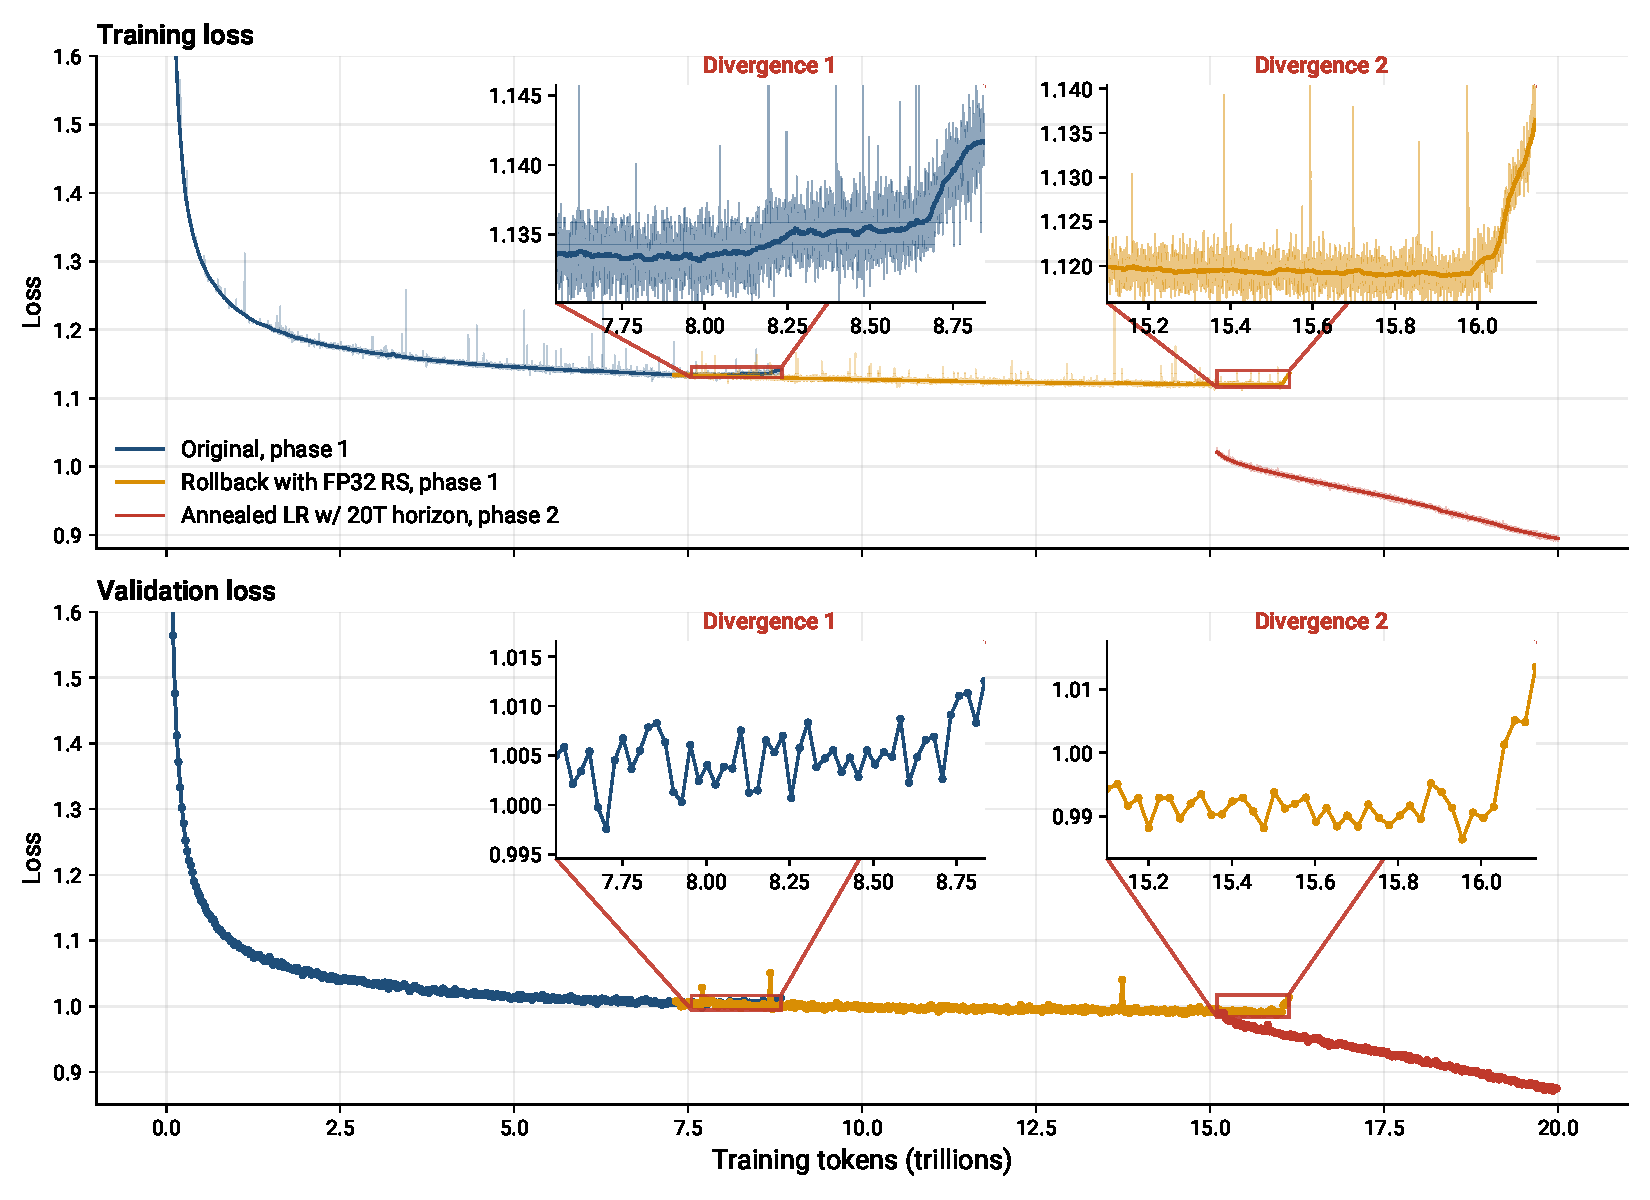
\includegraphics[width=\linewidth]{figures/loss_vs_tokens_full.pdf}
    \caption{Training and validation loss versus number of tokens. Two separate runs with ``phase 1'' data (``Original'' and ``Rollback with FP32 RS'') are shown in different colors; both resulted in loss divergences. Figure insets show zoomed-in versions of each divergence. ``Rollback with FP32 RS'' was obtained by starting from a checkpoint in the original run before the first loss divergence and using the original FP32 gradient reduction recipe.} \label{fig:loss_vs_tokens_full}
\end{figure*}


During pretraining, we observed two instances of training divergence characterized by simultaneous increases in both the training cross-entropy loss and \texttt{wgrad} L2 norm.  These are shown in Figure~\ref{fig:loss_vs_tokens_full}.


\begin{figure*}[!ht]
    \centering
    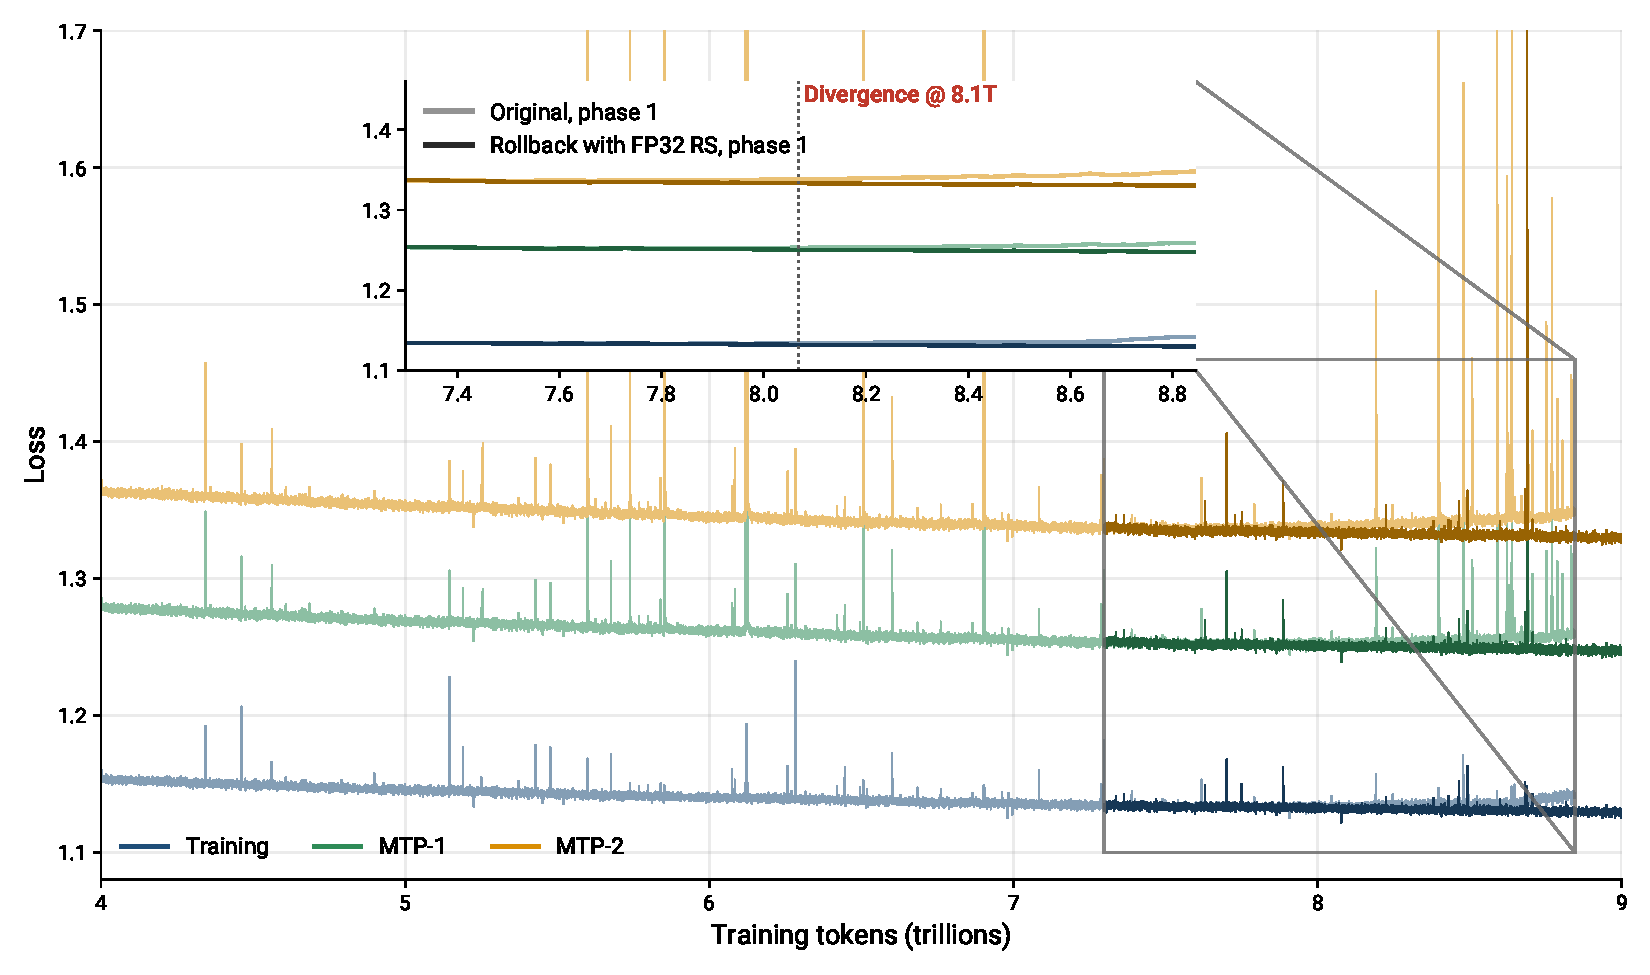
\includegraphics[width=\linewidth]{figures/loss_vs_tokens_divergence1_mtp.pdf}
    \caption{Training (cross-entropy loss for next token), MTP-1 and MTP-2 loss versus number of tokens around the region of the first divergence shown in Figure~\ref{fig:loss_vs_tokens_full}. MTP-2 loss diverges first with frequent large spikes.}
    \label{fig:loss_vs_tokens_divergence1_mtp}
\end{figure*}

\subsubsection*{Divergence 1: Local Gradient Accumulation Precision for Output Layer}

The first divergence, which occurred at around 8T tokens, was attributed to a reduction in local gradient accumulation precision for the output layer from FP32 to BF16 (in a bid to move data-parallel gradient reductions to BF16 over the wire as a throughput optimization). As mentioned in \S\ref{sec:architecture} and \S\ref{sec:hyperparameters}, \ourmodel uses 2 MTP blocks with a MTP loss scaling factor of 0.1 (0.05 for each MTP block); as a result, the MTP blocks' \texttt{wgrad} contribution to the shared output layer is essentially lost when using BF16, which has only 7 mantissa bits. Figure~\ref{fig:loss_vs_tokens_divergence1_mtp} shows MTP-2 loss started spiking / diverging before training (and validation) loss. Rolling back to an earlier checkpoint and moving back to the full FP32 gradient reduction recipe re-stabilized training (as shown in Figure~\ref{fig:loss_vs_tokens_full}).

\subsubsection*{Divergence 2: Undetermined}

\begin{figure*}[!ht]
    \centering
    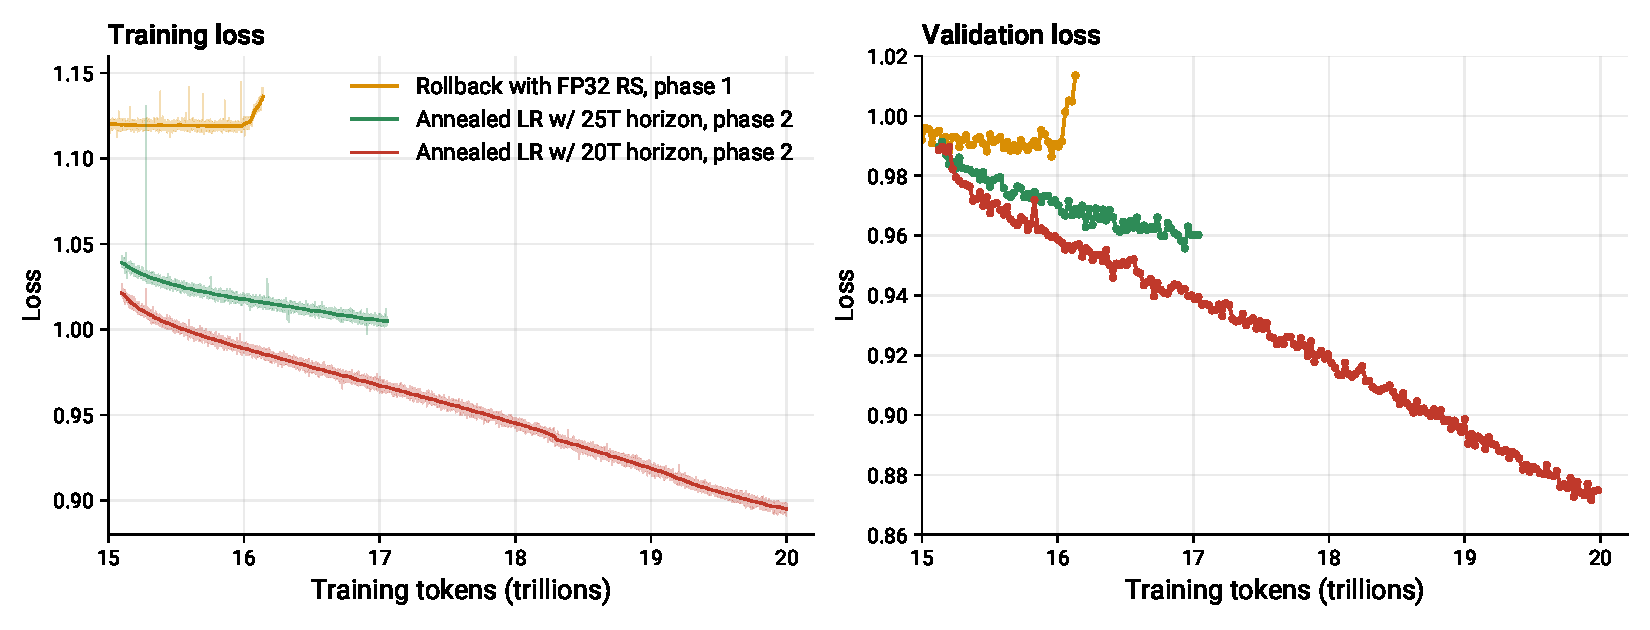
\includegraphics[width=\linewidth]{figures/loss_vs_tokens_divergence2.pdf}
    \caption{Training and validation loss around the second divergence (shown in Figure~\ref{fig:loss_vs_tokens_full}) for the original run that diverged (``Rollback with FP32 RS''), and two runs with early LR annealing targeting different token horizons after rewinding to a pre-divergence checkpoint (around 15T tokens).}
    \label{fig:loss_vs_tokens_divergence2}
\end{figure*}


\begin{figure}[!htp]
  \centering
  % Use subfigures to place them side-by-side
  \begin{subfigure}[b]{0.49\columnwidth}
    \centering
    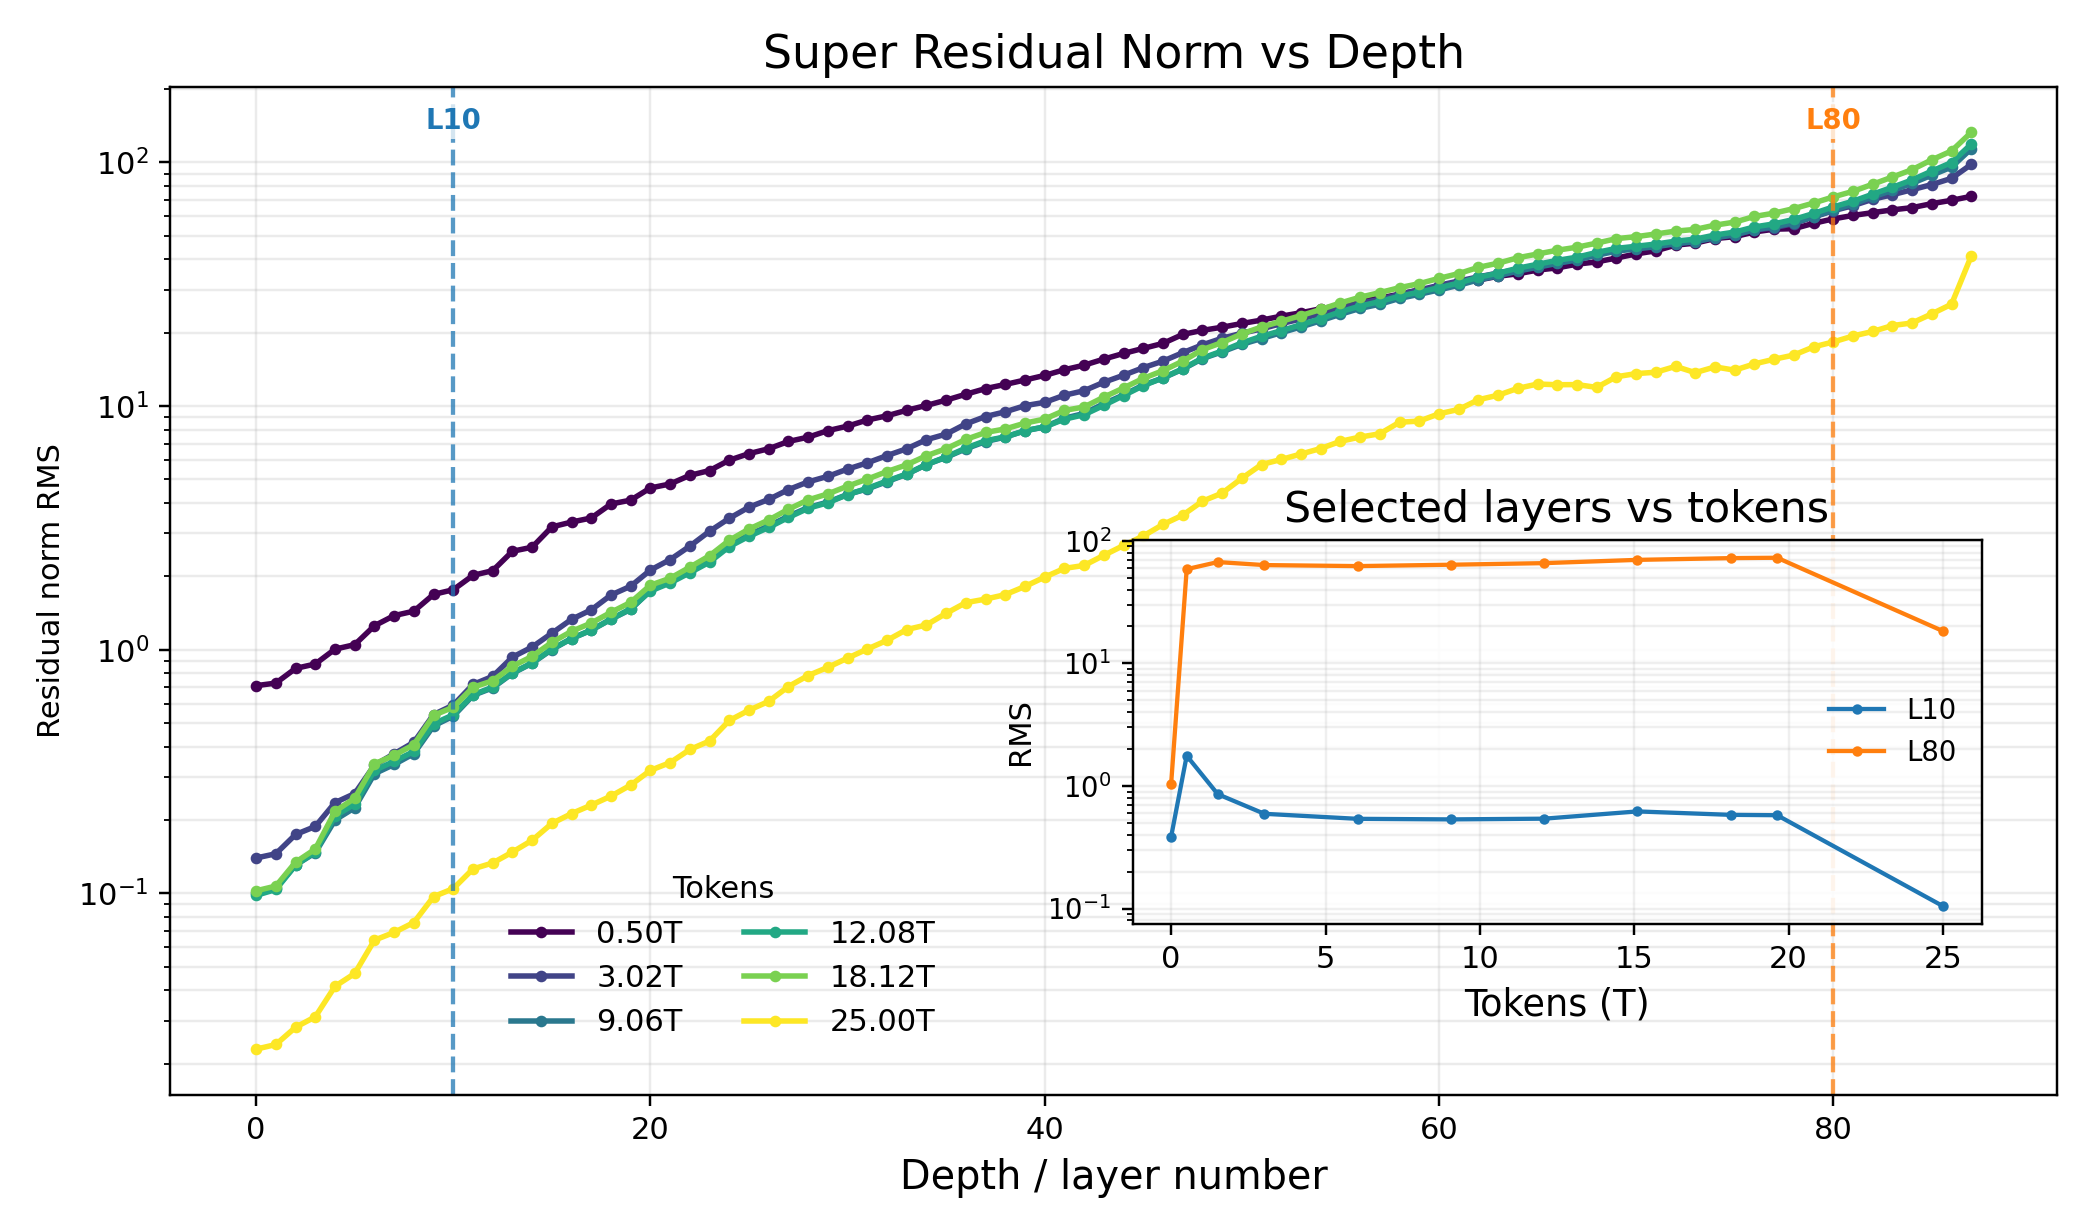
\includegraphics[width=\columnwidth]{figures/super_residual_norm_vs_depth.png}
    \caption{Nemotron-3-Super.}
    \label{fig:super_residual_norm}
  \end{subfigure}
  \hfill % Adds space between the figures
  \begin{subfigure}[b]{0.49\columnwidth}
    \centering
    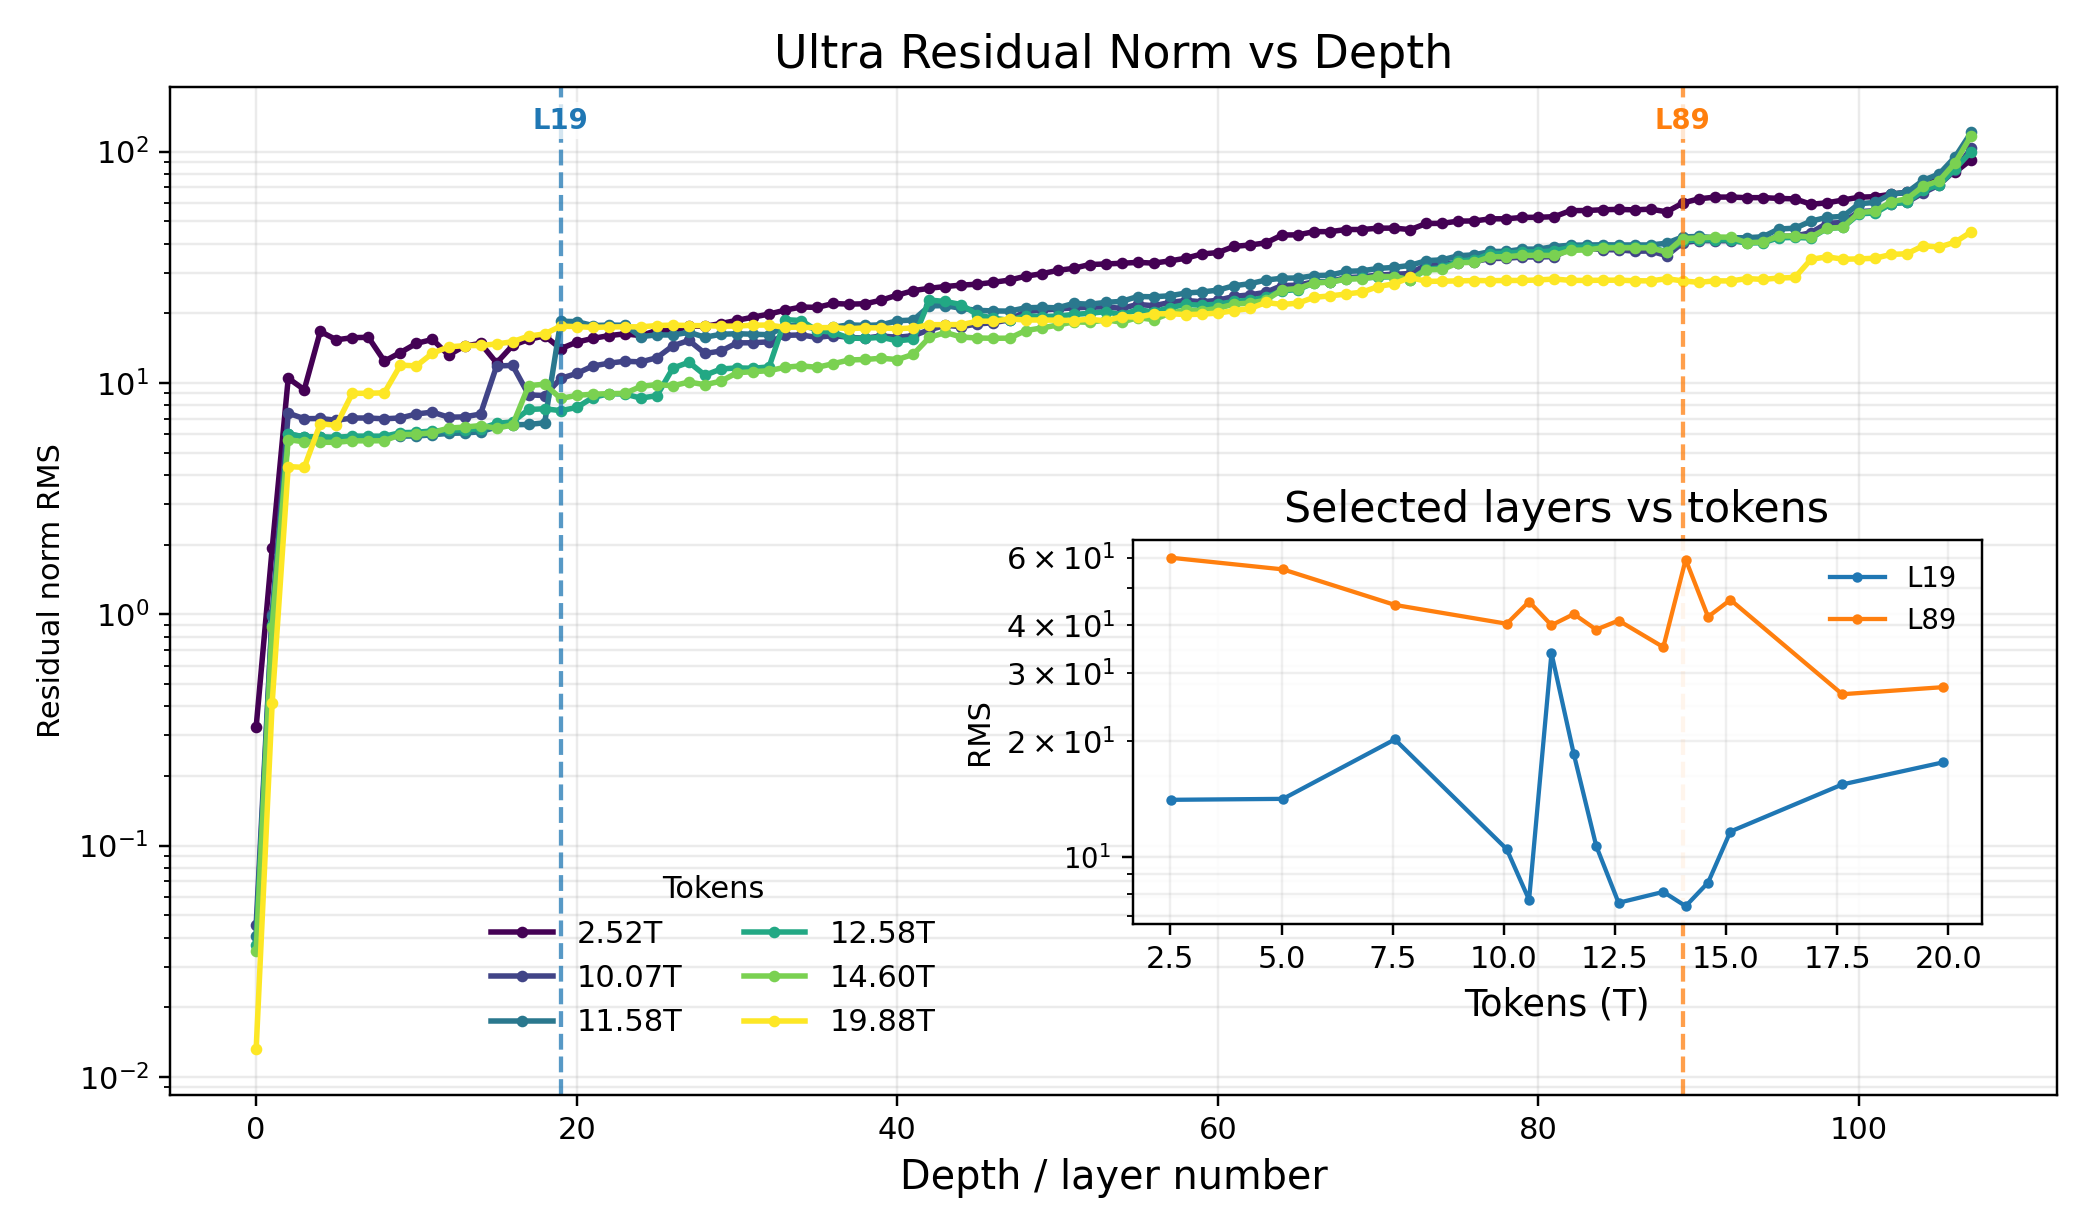
\includegraphics[width=\columnwidth]{figures/ultra_residual_norm_vs_depth.png}
    \caption{Nemotron-3-Ultra.}
    \label{fig:ultra_residual_norm}
  \end{subfigure}

  \vspace{1em} 

  \caption{Residual activation norm growth during training for Super and Ultra. The early layers for Super had increasing and then decreasing residual norms, with eventual stabilization. Later layers are characterized by norm growth. For Ultra, however, early layer residual norms started spiking about 7.5T tokens into training, with drastic spiking happening around 11T tokens, indicating increasing training instability.}
  \label{fig:super_ultra_residual_norms}
\end{figure}

For the second training divergence which occurred around $16$T tokens, we found through ablations that starting learning rate annealing (both a 5T and 10T decay) immediately after rolling back to the 15T token checkpoint mitigates divergence (Figure~\ref{fig:loss_vs_tokens_divergence2}). We eventually made the practical decision to cut the total pretraining token horizon down to 20T tokens.

To better understand the \emph{cause} of divergence, we studied the behavior of different model tensors across the full pretraining token horizon, and also between Super and Ultra. While we could not find a smoking gun that caused this instability, we found two interesting phenomena:

\paragraph{1. Imbalanced and Dead Experts.} As one possible proxy for pretraining health, the distribution of tokens across the available experts within the Mixture-of-Experts (MoE) layers can be continuously monitored. When a model begins to diverge or experience optimization difficulties, the routing mechanism often degrades, leading to severe token skew. In extreme cases, this results in ``dead experts'' that receive zero or near-zero tokens and effectively drop out of the learning process.
To quantify expert imbalance, we measure the MaxVio metric \citep{deepseekai2025deepseekv3technicalreport} which calculates the peak load on any single expert compared to the perfectly balanced mean. 

$\texttt{MaxVio} = \frac{\max_{1 \le i \le E} (T_i)}{\mu}$, where $E$ is the total number of experts, $T_i$ is the total number of tokens routed to expert $i$, and $\mu$ is the mean number of tokens per expert (calculated as $\frac{\sum T_i}{E}$).

We note that the maximum attainable MaxVio is $\text{MaxVio}_{\text{max}} = \frac{E}{k}$. For \ourmodel and Super, this gives us $\text{MaxVio}_{\text{max}} = 23.27$, while for Nano, it is $21.33$. 

We calculated MaxVio on 20 iterations worth of tokens (from both training and validation datasets) per checkpoint, for a total of 500M tokens. Across Nemotron-3 Nano, Super and Ultra, we observed that MaxVio on the training data was always lower than on the validation data over the course of pretraining. For Nano, the value was generally $\approx 1.3$ for training and $\approx 5$ for validation; for Super, it was $\approx 2$ and $\approx 6$, respectively. For Ultra, routing started balanced, with the median (across layers) MaxVio being $1.2$ and the maximum being $4.8$ (first MoE layer). As training progressed, expert routing became increasingly unbalanced; the median layer's MaxVio stayed around $1.2$ but the maximum kept increasing to $\approx 12$ by 12T tokens (again first layer). Although not causal by itself, MaxVio seems  correlated with training instability.

\paragraph{2. Imbalanced Residual Stream Activation Norms.} We found residual norms differed by 3 orders of magnitude across model depth for Super and 4 orders of magnitude for Ultra. Additionally, the dynamics of residual norms in \ourmodel were qualitatively different from what was observed during Nano and Super pretraining, as shown in Figure~\ref{fig:super_ultra_residual_norms}. For those models, residual norms in the early layers would increase, and then decrease and stabilize. Later layers had their residual norms slowly increase during training. For Ultra, residual norms initially followed this pattern, but norms in the early layers started rising around 7.5T pretraining tokens, with large residual norm spikes happening around 11T tokens, indicating poor signal propagation.


